\chapter{Asam dan Basa: Ka dan pKa}\label{ch:g12:ka-and-pka}

Banyak semut mempertahankan diri dengan asam metanoat, yang terasa
membakar di kulit. Asam metanoat adalah \omterm{def:g11:functional-groups:carboxylic-acid}{asam karboksilat} yang kecil.
Asam klorida dengan konsentrasi yang sama akan membakar jauh lebih
hebat. Keduanya asam; keduanya menghasilkan larutan dengan \omterm{def:g9:acids-bases-ph:ph}{pH} di bawah
7; tetapi keduanya tidak bersifat asam dengan cara yang sama. Untuk
menggambarkan sebuah asam secara lengkap, diperlukan dua bilangan:
berapa banyak asam itu, yaitu konsentrasinya, dan seberapa mudah asam
itu melepaskan \omterm{def:g9:ions:ion}{ion} hidrogennya, yaitu \omterm{def:g12:ka-and-pka:ka}{tetapan keasamannya}.

\begin{recall}
\omterm{def:g9:acids-bases-ph:acidic}{Larutan asam}, basa, dan netral; skala \omterm{def:g9:acids-bases-ph:ph}{pH}, dari 0 sampai 14, yang makin
rendah jika \omterm{def:g9:ions:ion}{ion} hidrogennya makin banyak (\cref{ch:g9:acids-bases-ph}).
\omterm{def:g12:equilibrium:quotient}{Kuosien reaksi} $Q$ dan \omterm{def:g12:equilibrium:constant}{tetapan kesetimbangan} $K$
(\cref{ch:g12:equilibrium}). \omterm{def:g12:curly-arrows:curly-arrow}{Panah lengkung} memperlihatkan perpindahan
sepasang \omterm{def:g9:inside-the-atom:nucleus}{elektron} (\cref{ch:g12:curly-arrows}).
\end{recall}

\begin{omfigure}
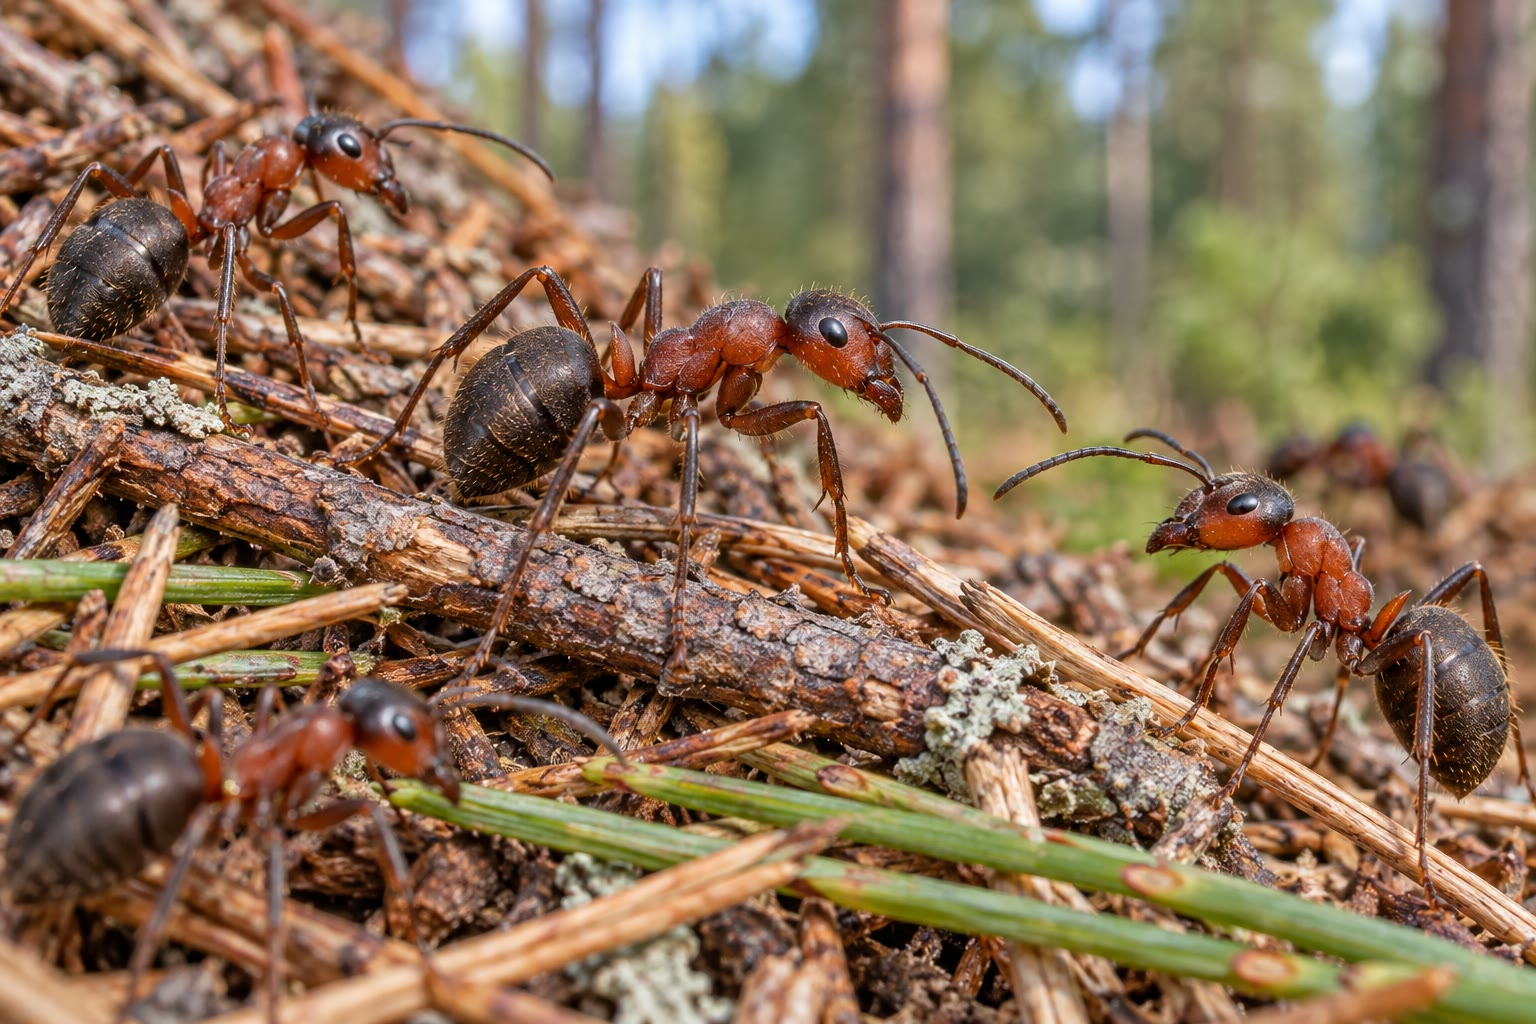
\includegraphics[width=0.45\linewidth]{images/book1/ai/g12-red-ants.jpg}

{\small Semut kayu: seperti banyak semut lain, semut ini mempertahankan
diri dengan asam metanoat.}
\end{omfigure}

\section{Asam dan basa Brønsted}

\begin{definition}[Asam dan basa Brønsted, pasangan asam--basa]\label{def:g12:ka-and-pka:bronsted}
Yang disebut \emph{asam Brønsted}\index{asam Brønsted} adalah spesies
yang mampu memberikan \omterm{def:g9:ions:ion}{ion} hidrogen \ce{H+}; \emph{basa
Brønsted}\index{basa Brønsted} adalah spesies yang mampu menerimanya.
Sebuah asam HA dan basa \ce{A-} yang terbentuk ketika asam itu
kehilangan \ce{H+} membentuk sebuah
\emph{pasangan asam--basa}\index{pasangan asam--basa}, yang ditulis
\ce{HA}/\ce{A-}: $\ce{HA} \rightleftharpoons \ce{A-} + \ce{H+}$.
\end{definition}

\begin{definition}[Ion oksonium, amfolit]\label{def:g12:ka-and-pka:oxonium}
Di dalam air, \omterm{def:g9:ions:ion}{ion} hidrogen tidak pernah sendirian: \omterm{def:g9:ions:ion}{ion} itu diambil oleh
sebuah \omterm{def:g7:atoms-and-molecules:molecule}{molekul} air, sehingga terbentuk \emph{ion
oksonium}\index{ion oksonium} \ce{H3O+}. Spesies yang merupakan asam
dari satu pasangan dan basa dari pasangan lain disebut
\emph{amfolit}\index{amfolit}; air adalah salah satunya, asam dari
pasangan \ce{H2O}/\ce{OH-} dan basa dari pasangan \ce{H3O+}/\ce{H2O}.
\end{definition}

\begin{example}[Asam di dalam air]\label{ex:g12:ka-and-pka:acid-water}
Ketika asam etanoat \omterm{def:g2:mixing-and-dissolving:dissolve}{larut}, sepasang \omterm{def:g9:inside-the-atom:nucleus}{elektron} bebas sebuah \omterm{def:g7:atoms-and-molecules:molecule}{molekul} air
mengambil hidrogen dari \ce{O-H}-nya, dan pasangan \omterm{def:g9:inside-the-atom:nucleus}{elektron} \ce{O-H}
tetap pada oksigen asam itu:
\[
  \ce{CH3COOH + H2O <=> CH3COO- + H3O+} .
\]
Dua pasangan bertukar \omterm{def:g9:ions:ion}{ion} hidrogen: \ce{CH3COOH}/\ce{CH3COO-}
memberikannya, \ce{H3O+}/\ce{H2O} menerimanya. Mulai sekarang, \omterm{def:g9:ions:ion}{ion}
hidrogen pada bab-bab sebelumnya ditulis \ce{H3O+} setiap kali air
menjadi \omterm{def:g6:solutions-and-solubility:solute}{pelarutnya}.
\end{example}

\begin{omfigure}
\setchemfig{atom sep=2em}
\chemfig{H_3C-C(=[2]O)-O-[@{oh}]@{h}H}\qquad
\chemfig{@{ow}\charge{90=\:,270=\:}{O}(-[:150]H)-[:210]H}
\qquad$\longrightarrow$\qquad
\chemfig{H_3C-C(=[2]O)-\charge{90=\:,0=\:,270=\:}{O}^{-}}\quad$+$\quad\ce{H3O+}
\chemmove{
  \draw[->, thick, omProp, shorten <=4pt, shorten >=3pt]
    ($(ow)+(0,0.25)$) .. controls +(110:9mm) and +(60:9mm) .. (h);
  \draw[->, thick, omDef, shorten <=2pt, shorten >=4pt]
    (oh) .. controls +(-90:7mm) and +(-60:6mm) .. ($(oh)+(-0.3,-0.2)$);}

{\small \omterm{def:g9:ions:ion}{Ion} hidrogen berpindah dari asam ke air: sepasang \omterm{def:g9:inside-the-atom:nucleus}{elektron} bebas
air membentuk ikatan \ce{O-H} yang baru (jingga), dan pasangan \omterm{def:g9:inside-the-atom:nucleus}{elektron}
\ce{O-H} yang lama tetap pada oksigen \omterm{def:g9:ions:ion}{ion} etanoat (biru).}
\end{omfigure}

\begin{history}[Dari Arrhenius ke Brønsted, 1887--1923]
Pada tahun 1887 Svante Arrhenius mengusulkan bahwa asam menghasilkan \omterm{def:g9:ions:ion}{ion}
hidrogen di dalam air dan basa menghasilkan \omterm{def:g9:ions:ion}{ion} hidroksida. Pada tahun
1923 Johannes Brønsted, dan secara terpisah Thomas Lowry, memperluas
gagasan itu: asam adalah spesies apa pun yang memberikan \omterm{def:g9:ions:ion}{ion} hidrogen,
basa adalah spesies apa pun yang menerimanya, di dalam air atau tidak.
\omterm{def:g7:atoms-and-molecules:molecule}{Molekul} amonia, yang tidak mengandung hidroksida, menjadi basa seperti
basa lainnya.
\end{history}

\begin{omfigure}
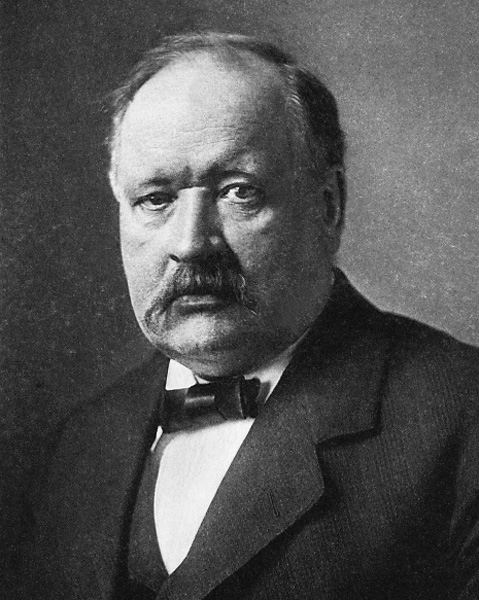
\includegraphics[width=0.22\linewidth]{images/book1/arrhenius.jpg}

{\small Svante Arrhenius (1859--1927).}
\end{omfigure}

\section{pH secara kuantitatif}

\begin{definition}[pH secara tepat]\label{def:g12:ka-and-pka:ph-log}
Dalam \omterm{def:g6:solutions-and-solubility:solute}{larutan berair} yang encer, \omterm{def:g9:acids-bases-ph:ph}{pH} didefinisikan oleh
\[
  \mathrm{pH} = -\log\frac{[\ce{H3O+}]}{c^\circ},
  \qquad\text{yaitu}\qquad
  [\ce{H3O+}] = c^\circ \times 10^{-\mathrm{pH}} ,
\]
dengan $\log$ logaritma desimal.
\end{definition}

\begin{proposition}[Pengenceran sepuluh kali, satu satuan]\label{prop:g12:ka-and-pka:dilution}
Jika $[\ce{H3O+}]$ dibagi 10, \omterm{def:g9:acids-bases-ph:ph}{pH} naik 1; jika dikalikan 10, \omterm{def:g9:acids-bases-ph:ph}{pH} turun 1.
\end{proposition}

\begin{proof}
$-\log\big([\ce{H3O+}]/10c^\circ\big) = -\log\big([\ce{H3O+}]/c^\circ\big)
+ \log 10 = \mathrm{pH} + 1$.
\end{proof}

\begin{definition}[Asam dan basa kuat dan lemah]\label{def:g12:ka-and-pka:strong-acid}
Yang disebut \emph{asam kuat}\index{asam kuat} adalah asam yang bereaksi
tuntas dengan air: tidak ada asam yang tetap dalam bentuk semula di
dalam larutan. Yang disebut \emph{asam lemah}\index{asam lemah} adalah
asam yang bereaksi sebagian:
reaksinya dengan air mencapai kesetimbangan. Demikian pula,
\emph{basa kuat}\index{basa kuat} bereaksi tuntas dengan air,
\emph{basa lemah}\index{basa lemah} bereaksi sebagian.
\end{definition}

\begin{proposition}[pH asam kuat]\label{prop:g12:ka-and-pka:strong}
Larutan \omterm{def:g12:ka-and-pka:strong-acid}{asam kuat} berkonsentrasi $c$ (yang tidak terlalu encer) memiliki
$[\ce{H3O+}] = c$ dan $\mathrm{pH} = -\log(c/c^\circ)$.
\end{proposition}

\begin{proof}
Reaksi \ce{HA + H2O -> A- + H3O+} berlangsung tuntas: setiap \omterm{def:g7:atoms-and-molecules:molecule}{molekul}
asam menghasilkan satu \omterm{def:g12:ka-and-pka:oxonium}{ion oksonium}. \omterm{def:g9:ions:ion}{Ion-ion} yang berasal dari air
sendiri dapat diabaikan selama $c$ jauh lebih besar daripada
\qty{e-7}{mol/L}.
\end{proof}

\begin{example}[Asam klorida]\label{ex:g12:ka-and-pka:hcl}
Asam klorida \qty{0.010}{mol/L}: $[\ce{H3O+}] = \qty{0.010}{mol/L}$
dan $\mathrm{pH} = -\log 0.010 = 2.0$. Setelah diencerkan sepuluh kali,
\omterm{def:g9:acids-bases-ph:ph}{pH} 3.0.
\end{example}

\section{Air dan hasil kali ionnya}


\begin{definition}[Hasil kali ion air]\label{def:g12:ka-and-pka:ionic-product}
Air bereaksi sangat sedikit dengan dirinya sendiri,
\ce{2H2O <=> H3O+ + OH-}. \omterm{def:g12:equilibrium:constant}{Tetapan kesetimbangan} reaksi ini disebut
\emph{hasil kali ion air}\index{hasil kali ion air}:
\[
  K_e = \frac{[\ce{H3O+}]\,[\ce{OH-}]}{(c^\circ)^2},
  \qquad pK_e = -\log K_e .
\]
\end{definition}

\begin{proposition}[Air netral dan basa kuat]\label{prop:g12:ka-and-pka:ke}
% ledger: ke:25C
Pada \qty{25}{\celsius}, $K_e = \num{1.0e-14}$ dan $pK_e = 14.0$. Dalam
air murni, $[\ce{H3O+}] = [\ce{OH-}] = \qty{1.0e-7}{mol/L}$: \omterm{def:g9:acids-bases-ph:ph}{pH} 7.0.
\omterm{def:g12:ka-and-pka:strong-acid}{Basa kuat} berkonsentrasi $c$ menghasilkan $[\ce{OH-}] = c$, sehingga
$[\ce{H3O+}] = K_e (c^\circ)^2 / c$ dan $\mathrm{pH} = 14.0 + \log(c/c^\circ)$.
\end{proposition}

\begin{proof}
Dalam air murni, kedua \omterm{def:g9:ions:ion}{ion} terbentuk berpasangan, sehingga jumlahnya
sama, dan hasil kalinya $\num{1.0e-14}$: masing-masing
\qty{1.0e-7}{mol/L}. Untuk basa, $K_e$ tetap berlaku dalam larutan:
$-\log([\ce{H3O+}]/c^\circ) = -\log K_e + \log(c/c^\circ)$.
\end{proof}

\begin{example}[Natrium hidroksida]\label{ex:g12:ka-and-pka:naoh}
Natrium hidroksida \qty{0.010}{mol/L}: $[\ce{OH-}] = 0.010$, jadi
$[\ce{H3O+}] = \num{1.0e-14}/0.010 = \qty{1.0e-12}{mol/L}$ dan \omterm{def:g9:acids-bases-ph:ph}{pH} 12.0.
\end{example}

\section{Tetapan keasaman}

\begin{definition}[Tetapan keasaman, $pK_a$]\label{def:g12:ka-and-pka:ka}
Yang disebut \emph{tetapan keasaman}\index{tetapan keasaman} $K_a$
sebuah pasangan \ce{HA}/\ce{A-} adalah \omterm{def:g12:equilibrium:constant}{tetapan kesetimbangan} reaksi
asam itu dengan air, \ce{HA + H2O <=> A- + H3O+}:
\[
  K_a = \frac{[\ce{A-}]\,[\ce{H3O+}]}{[\ce{HA}]\,c^\circ} .
\]
Nilai \emph{pKa}\index{pKa} pasangan itu adalah
$pK_a = -\log K_a$.
\end{definition}

\begin{proposition}[Makin kecil $pK_a$, makin kuat asamnya]\label{prop:g12:ka-and-pka:compare}
Dari dua \omterm{def:g12:ka-and-pka:strong-acid}{asam lemah} dengan konsentrasi yang sama, asam dengan $K_a$ yang
lebih besar, yaitu $pK_a$ yang lebih kecil, lebih banyak bereaksi
dengan air dan memberikan \omterm{def:g9:acids-bases-ph:ph}{pH} yang lebih rendah; basa konjugatnya lebih
lemah.
\end{proposition}

\begin{proof}
$K_a$ yang lebih besar berarti lebih banyak \ce{A-} dan \ce{H3O+} pada
kesetimbangan untuk \ce{HA} yang sama. Basa \ce{A-} dari pasangan yang
mudah melepaskan \omterm{def:g9:ions:ion}{ion} hidrogennya enggan menerimanya kembali.
\end{proof}

\begin{omfigure}
\begin{tikzpicture}[font=\small, y=0.55cm]
  % ledger: pka:methanoic, pka:ethanoic, pka:benzoic, pka:ascorbic1, ka:HF, ka:H2CO3, ka:HCO3, kb:NH3, ke:25C
  \draw[->, thick] (0,0) -- (0,14.8) node[above] {$pK_a$};
  \foreach \k in {0,2,4,6,8,10,12,14} \draw (-0.1,\k) -- (0.1,\k) node[right, font=\scriptsize] {\k};
  \node[font=\footnotesize\bfseries, anchor=south] at (-3.0,14.3) {asam};
  \node[font=\footnotesize\bfseries, anchor=south] at (3.0,14.3) {basa};
  \foreach \p/\yl/\acid/\base in {3.19/2.9/{\ce{HF}}/{\ce{F-}},
      3.74/3.6/{\ce{HCOOH}}/{\ce{HCOO-}}, 4.04/4.3/{asam askorbat}/{askorbat},
      4.20/5.0/{\ce{C6H5COOH}}/{\ce{C6H5COO-}}, 4.76/5.7/{\ce{CH3COOH}}/{\ce{CH3COO-}},
      6.37/6.9/{\ce{CO2,H2O}}/{\ce{HCO3-}}, 9.26/9.26/{\ce{NH4+}}/{\ce{NH3}},
      10.33/10.4/{\ce{HCO3-}}/{\ce{CO3^{2-}}}} {
    \draw[omDef] (-0.25,\p) -- (0.25,\p);
    \draw[black!40] (-0.25,\p) -- (-1.1,\yl);
    \draw[black!40] (0.25,\p) -- (1.1,\yl);
    \node[anchor=east, font=\scriptsize] at (-1.15,\yl) {\acid};
    \node[anchor=west, font=\scriptsize] at (1.15,\yl) {\base};
  }
  \draw[->, omThm, thick] (-4.6,13) -- (-4.6,1);
  \node[omThm, rotate=90, font=\footnotesize] at (-4.95,7) {asam makin kuat};
  \draw[->, omMeth, thick] (4.6,1) -- (4.6,13);
  \node[omMeth, rotate=90, font=\footnotesize] at (4.95,7) {basa makin kuat};
\end{tikzpicture}

{\small Beberapa pasangan yang ditempatkan menurut $pK_a$-nya pada
\qty{25}{\celsius}, asam di kiri, basanya di kanan. Makin rendah letak
sebuah pasangan pada skala, makin kuat asamnya; makin tinggi, makin kuat
basanya.}
\end{omfigure}


\begin{method}[pH asam lemah]\label{met:g12:ka-and-pka:weak}
Untuk \omterm{def:g12:ka-and-pka:strong-acid}{asam lemah} berkonsentrasi $c$ dengan tetapan $K_a$:
\begin{enumerate}
  \item Tuliskan \omterm{def:g10:reaction-progress-table:extent}{tabel kemajuan} \ce{HA + H2O <=> A- + H3O+} per liter,
        dengan $x = [\ce{H3O+}]$: $[\ce{HA}] = c - x$, $[\ce{A-}] = x$
        (\omterm{def:g9:ions:ion}{ion-ion} air sendiri diabaikan).
  \item Selesaikan $\dfrac{x^2}{(c - x)\,c^\circ} = K_a$, yaitu persamaan
        kuadrat $x^2 + K_a c^\circ x - K_a c^\circ c = 0$, dengan
        mempertahankan akar positifnya.
  \item $\mathrm{pH} = -\log(x/c^\circ)$; periksalah bahwa $x$ jauh lebih
        besar daripada \qty{e-7}{mol/L}.
\end{enumerate}
\end{method}

\begin{example}[Asam etanoat \texorpdfstring{\qty{0.010}{mol/L}}{0.010 \omterm{def:g10:the-mole:amount}{mol}/L}]\label{ex:g12:ka-and-pka:acetic}
% ledger: pka:ethanoic
$pK_a = 4.76$, jadi $K_a = 10^{-4.76} = \num{1.74e-5}$. Lalu
$x^2 + \num{1.74e-5}\,x - \num{1.74e-7} = 0$ memberikan
$x = \qty{4.1e-4}{mol/L}$ dan \omterm{def:g9:acids-bases-ph:ph}{pH} 3.39. Hanya $\num{4.1e-4}/0.010 =
\qty{4.1}{\percent}$ asam yang telah bereaksi dengan air; asam klorida
dengan konsentrasi yang sama, \omterm{def:g9:acids-bases-ph:ph}{pH} 2.0, telah bereaksi seluruhnya.
\end{example}

\begin{omfigure}
\begin{tikzpicture}[font=\small]
  \fill[omThm!45] (0,1.3) rectangle (8,2.0);
  \node[anchor=east] at (-0.1,1.65) {\ce{HCl}, \qty{0.010}{mol/L}};
  \node[white, font=\small\bfseries] at (4,1.65) {\ce{H3O+} + \ce{Cl-}: \qty{100}{\percent}};
  \fill[omDef!35] (0,0) rectangle (7.67,0.7);
  \fill[omThm!45] (7.67,0) rectangle (8,0.7);
  \node[anchor=east] at (-0.1,0.35) {\ce{CH3COOH}, \qty{0.010}{mol/L}};
  \node at (3.8,0.35) {\ce{CH3COOH} tetap utuh: \qty{95.9}{\percent}};
  \draw[<-, omThm] (7.85,0.75) -- (8.4,1.1) node[right, font=\footnotesize] {\qty{4.1}{\percent} terionisasi};
\end{tikzpicture}

{\small Apa yang terjadi pada \omterm{def:g12:ka-and-pka:strong-acid}{asam kuat} dan \omterm{def:g12:ka-and-pka:strong-acid}{asam lemah} dengan
konsentrasi yang sama: \omterm{def:g12:ka-and-pka:strong-acid}{asam kuat} seluruhnya berubah menjadi \omterm{def:g9:ions:ion}{ion}, \omterm{def:g12:ka-and-pka:strong-acid}{asam
lemah} hampir tidak. Itulah sebab perbedaan \omterm{def:g9:acids-bases-ph:ph}{pH-nya}, 2.0 dibandingkan
3.4.}
\end{omfigure}

\begin{safety}{\ghs[0.75cm]{GHS02}\ghs[0.75cm]{GHS05}\ghs[0.75cm]{GHS06}\ghs[0.75cm]{GHS07}}
% ledger: ghs:formic-acid
Asam metanoat pekat mudah menyala, menyebabkan luka bakar parah pada
kulit dan mata, dan uapnya beracun. Asam ini hanya ditangani oleh guru,
di dalam lemari asam; larutan encer dalam latihan tetap memerlukan
kacamata pelindung.
\end{safety}

\section{Latihan}

\begin{exercise}[$\star$]\label{exo:g12:ka-and-pka:1}
Berikan basa konjugat dari: \ce{HCOOH}, \ce{NH4+}, \ce{H2O}, \ce{HCO3-};
dan asam konjugat dari: \ce{NH3}, \ce{OH-}, \ce{H2O}, \ce{HCO3-}.
Spesies mana yang merupakan \omterm{def:g12:ka-and-pka:oxonium}{amfolit}?
\end{exercise}

\begin{exercise}[$\star$]\label{exo:g12:ka-and-pka:2}
Hitung \omterm{def:g9:acids-bases-ph:ph}{pH} asam klorida \qty{0.10}{mol/L}, \qty{0.0010}{mol/L}, dan
\qty{5.0e-3}{mol/L}.
\end{exercise}

\begin{exercise}[$\star$]\label{exo:g12:ka-and-pka:3}
Sebuah larutan memiliki \omterm{def:g9:acids-bases-ph:ph}{pH} 4.5. Hitung $[\ce{H3O+}]$. Sebuah larutan
memiliki \omterm{def:g9:acids-bases-ph:ph}{pH} 11.2: hitung $[\ce{H3O+}]$ dan $[\ce{OH-}]$ pada
\qty{25}{\celsius}.
\end{exercise}

\begin{exercise}[$\star$]\label{exo:g12:ka-and-pka:4}
Tuliskan reaksi dengan air dan ungkapan $K_a$ untuk asam metanoat dan
untuk \omterm{def:g9:ions:ion}{ion} amonium.
\end{exercise}

\begin{exercise}[$\star$]\label{exo:g12:ka-and-pka:5}
Manakah asam yang lebih kuat: asam metanoat ($pK_a = 3.74$) atau asam
etanoat ($pK_a = 4.76$)? Manakah basa yang lebih kuat: \ce{HCOO-} atau
\ce{CH3COO-}?
\end{exercise}

\begin{exercise}[$\star\star$]\label{exo:g12:ka-and-pka:6}
Larutan \omterm{def:g12:ka-and-pka:strong-acid}{asam lemah} HA \qty{0.050}{mol/L} memiliki \omterm{def:g9:acids-bases-ph:ph}{pH} 3.0. Hitung
$[\ce{A-}]$, $[\ce{HA}]$, lalu $K_a$ dan $pK_a$.
\end{exercise}

\begin{exercise}[$\star\star$]\label{exo:g12:ka-and-pka:7}
Hitung \omterm{def:g9:acids-bases-ph:ph}{pH} asam benzoat \qty{0.020}{mol/L} ($pK_a = 4.20$).
\end{exercise}

\begin{exercise}[$\star\star$]\label{exo:g12:ka-and-pka:8}
Hitung \omterm{def:g9:acids-bases-ph:ph}{pH} larutan natrium hidroksida \qty{2.0e-3}{mol/L}.
\end{exercise}

\begin{exercise}[$\star\star$]\label{exo:g12:ka-and-pka:9}
Dengan skala $pK_a$, urutkan asam-asam dari pasangan yang diperlihatkan,
dari yang terkuat sampai yang terlemah. Di mana letak \omterm{def:g12:ka-and-pka:strong-acid}{asam kuat} seperti
\ce{HCl}?
\end{exercise}

\begin{exercise}[$\star\star$]\label{exo:g12:ka-and-pka:10}
Karbon dioksida yang terlarut dalam air membuatnya sedikit asam
(pasangan \ce{CO2,H2O}/\ce{HCO3-}, $pK_a = 6.37$). Sebuah sampel air
hujan yang bersentuhan dengan \omterm{def:g4:air-a-mixture-of-gases:air}{udara} ternyata memiliki \omterm{def:g9:acids-bases-ph:ph}{pH} 5.6. Hitung
$[\ce{H3O+}]$, lalu bandingkan dengan air murni.
\end{exercise}

\begin{exercise}[$\star\star$]\label{exo:g12:ka-and-pka:11}
Tunjukkan bahwa untuk pasangan \ce{NH4+}/\ce{NH3}, $pK_a = pK_e - pK_b$,
dengan $K_b = \num{1.8e-5}$ tetapan reaksi \ce{NH3 + H2O <=> NH4+ + OH-}.
Hitung $pK_a$-nya.
\end{exercise}

\begin{exercise}[$\star\star\star$]\label{exo:g12:ka-and-pka:12}
Asam etanoat \qty{0.010}{mol/L} memiliki \omterm{def:g9:acids-bases-ph:ph}{pH} 3.39. Hitung \omterm{def:g9:acids-bases-ph:ph}{pH-nya} setelah
diencerkan sepuluh kali. Apakah \omterm{def:g9:acids-bases-ph:ph}{pH} itu naik satu satuan, seperti pada
\omterm{def:g12:ka-and-pka:strong-acid}{asam kuat}? Jelaskan.
\end{exercise}

\begin{exercise}[$\star\star\star$]\label{exo:g12:ka-and-pka:13}
\omterm{def:g9:ions:ion}{Ion} hidrogenkarbonat adalah \omterm{def:g12:ka-and-pka:oxonium}{amfolit}. Tuliskan kedua reaksinya dengan
air beserta tetapannya, dengan memakai skala $pK_a$. Manakah yang lebih
besar? Apa yang ditunjukkan hal itu tentang \omterm{def:g9:acids-bases-ph:ph}{pH} larutan natrium
hidrogenkarbonat?
\end{exercise}

\begin{exercise}[$\star\star\star$]\label{exo:g12:ka-and-pka:14}
Asam klorida \qty{1.0e-3}{mol/L} diencerkan seribu kali, lalu seribu
kali lagi. Sebuah aturan yang ceroboh memberikan \omterm{def:g9:acids-bases-ph:ph}{pH} 6, lalu \omterm{def:g9:acids-bases-ph:ph}{pH} 9.
Mengapa \omterm{def:g9:acids-bases-ph:ph}{pH} 9 tidak mungkin bagi asam yang diencerkan? \omterm{def:g9:acids-bases-ph:ph}{pH} berapa yang
didekati larutan yang sangat encer itu?
\end{exercise}

\begin{exercise}[$\star\star\star$]\label{exo:g12:ka-and-pka:15}
Asam askorbat (vitamin C, $pK_a = 4.04$, $M = \qty{176.0}{g/mol}$):
sebutir tablet \qty{500}{mg} dilarutkan dalam \qty{200}{mL} air. Hitung
\omterm{def:g9:acids-bases-ph:ph}{pH-nya} (perhitungkan hanya keasaman pertamanya).
\end{exercise}

\section{Soal: Bisa Semut}


\begin{problem}[{Soal akhir pekan --- berapa pH yang dihasilkan asam
metanoat bisa semut pada 0.010 mol/L, dan bagaimana soda kue meredakan
rasa terbakarnya?}]
\label{pb:g12:ka-and-pka:1}
% ledger: src:formic-ants, pka:methanoic, ka:H2CO3, ke:25C, aw:C, aw:H, aw:O
Asam metanoat, \ce{HCOOH}, terdapat dalam bisa semut. $pK_a$-nya pada
\qty{25}{\celsius} adalah 3.74. Kita mempelajari larutan
\qty{0.010}{mol/L} dan membandingkannya dengan asam klorida.

\medskip
\noindent\textbf{Bagian I --- Asamnya.}
\begin{enumerate}
  \item Gambarlah \omterm{def:g10:lewis-and-shape:lewis-structure}{struktur Lewis} asam metanoat dan lingkarilah hidrogen
        yang dilepaskannya.
  \item Tuliskan pasangannya dan reaksinya dengan air.
  \item Tuliskan $K_a$ dan hitung nilainya.
  \item Tempatkan pasangan itu pada skala $pK_a$: apakah asam metanoat
        lebih kuat atau lebih lemah daripada asam etanoat?
  \item Hitung massa asam metanoat dalam \qty{1.0}{L} larutan itu.
\end{enumerate}

\medskip
\noindent\textbf{Bagian II --- \omterm{def:g9:acids-bases-ph:ph}{pH-nya}.}
\begin{enumerate}[resume]
  \item Isilah \omterm{def:g10:reaction-progress-table:extent}{tabel kemajuan} per liter, dengan $x = [\ce{H3O+}]$.
  \item Tuliskan persamaan $Q_{eq} = K_a$.
  \item Selesaikan persamaan itu.
  \item Hitung \omterm{def:g9:acids-bases-ph:ph}{pH-nya}.
  \item Berapa bagian asam yang telah bereaksi dengan air?
  \item Periksalah bahwa \omterm{def:g9:ions:ion}{ion-ion} yang berasal dari air dapat diabaikan.
\end{enumerate}

\medskip
\noindent\textbf{Bagian III --- Perbandingan.}
\begin{enumerate}[resume]
  \item Berapa \omterm{def:g9:acids-bases-ph:ph}{pH} asam klorida \qty{0.010}{mol/L}?
  \item Berapa kali lebih banyak \omterm{def:g12:ka-and-pka:oxonium}{ion oksonium} yang dikandungnya
        dibandingkan larutan asam metanoat?
  \item Jelaskan perbedaannya, dengan memakai kata kuat dan lemah.
\end{enumerate}

\medskip
\noindent\textbf{Bagian IV --- Soda kue.}
\begin{enumerate}[resume]
  \item Soda kue adalah natrium hidrogenkarbonat. Tuliskan reaksi antara
        asam metanoat dan \omterm{def:g9:ions:ion}{ion} hidrogenkarbonat (reaksi itu menghasilkan
        metanoat dan \ce{CO2,H2O}).
  \item Tunjukkan bahwa tetapannya adalah
        $K = K_a(\ce{HCOOH}) / K_a(\ce{CO2,H2O})$, lalu hitung nilainya.
  \item Apakah reaksi itu menguntungkan? Gas apa yang terlihat?
  \item Mengapa basa yang jauh lebih lemah daripada hidroksida, seperti
        hidrogenkarbonat, lebih disukai untuk kulit?
  \item Nyatakan jawaban akhirnya: berapa \omterm{def:g9:acids-bases-ph:ph}{pH} larutan asam metanoat
        \qty{0.010}{mol/L}?
\end{enumerate}
\end{problem}
